\chapter{Implementierung} % DeepL korrigiert

In diesem Kapitel wird der Prozess der Implementierung der in Kapitel \ref{section:konzept} erarbeiteten Interaktionskonzepte in Prototypen dargelegt. 
Zunächst wird ein Überblick über die Entwicklungsumgebung gegeben, welche für die Entwicklung mit WebXR auf einer Meta Quest 3 eingerichtet wurde.
Im Anschluss erfolgt eine Beschreibung der Implementierung der Prototypen für jedes Interaktionskonzept, wobei einige technische Details erläutert werden.

\section{Entwicklungsumgebung für WebXR und Meta~Quest~3}

Die Entwicklung von WebXR-Anwendungen für die Meta Quest 3 erfordert eine spezielle Entwicklungsumgebung für einen effizienten Entwicklungsprozess.
Diese muss verschiedene Technologien und Tools miteinander kombinieren, um eine reibungslose Entwicklung und ein möglichst schnelles Testen der Anwendung zu gewährleisten.



Der erste Schritt besteht in der Anzeige der WebXR-Anwendung auf der Meta Quest 3. 
Im Vergleich zu \glqq{}normalen\grqq{} Webanwendungen ist dabei zu beachten, dass WebXR-Anwendungen ausschließlich über HTTPS aufgerufen werden können.
Das bedeutet, dass die Anwendung über HTTPS gehostet werden muss, um direkt vom Browser der Meta Quest 3 aufgerufen werden zu können.
Dafür existieren verschiedene Möglichkeiten, wie beispielsweise das Erstellen eines eigenen Zertifikats für den lokalen Entwicklungsrechner oder das Hosting der Anwendung auf einem Server mit HTTPS-Unterstützung.
Im Rahmen der Entwicklung dieser Bachelorarbeit wird die Anwendung jedoch -- wie auch in der Artikelserie des Taikonautenmagazins \autocite[Part 0/8]{taikonauten-magazine} empfohlen -- mit LocalTunnel gehostet, um die Anwendung direkt von der Meta Quest 3 aus testen zu können.
LocalTunnel generiert einen temporären HTTPS-Link, über den die Anwendung aufgerufen werden kann, ohne dass ein eigenes Zertifikat oder ein eigener Server erforderlich ist.
Dazu muss die Anwendung lediglich lokal auf dem Entwicklungsrechner ausgeführt werden und der LocalTunnel-Client gestartet sein, um einen temporären Link zu erstellen.
Um eine zusätzliche Sicherheit zu gewährleisten, muss beim Aufrufen der Seite die IP-Adresse des Entwicklungsrechners angegeben werden.
Auf diese Weise kann sichergestellt werden, dass ausschließlich der Entwickler die Anwendung testen kann.
Zudem wird so verhindert, dass Betrüger LocalTunnels nutzen, um HTTPS-Websites nachzuahmen.
Diese Eingabe muss in der Regel jedoch nur einmal nach jedem Neustart oder Crash gemacht werden, da der Link für die Dauer der Sitzung gespeichert wird.
Allerdings neigt der LocalTunnel dazu, regelmäßig abzustürzen, weshalb auch diese Lösung als suboptimal zu bewerten ist.

Der nächste Schritt, sofern ein Zugriff auf die WebXR-Anwendung mit der Meta Quest 3 besteht, umfasst die Anzeige von Entwickler-Tools und Debugging-Informationen der Meta Quest 3.
Diese Arbeit sowie die Prototypen wurden nahezu vollständig unter Linux entwickelt.
Für das Debuggen von Meta Geräten kann auf Windows die Meta Quest Developer Hub App (MQDH) genutzt werden, welche jedoch zum Zeitpunkt dieser Arbeit noch nicht auf Linux installiert werden kann.
Daher mussten für das Debuggen der Meta Quest 3 Umwege gefunden werden. \newline
Da die Meta Quest 3 auf Android basiert, besteht die Möglichkeit, auf dem Linux"=Entwicklungsrechner die Android Debug Bridge (ADB) zu installieren, um über USB eine Verbindung zur Meta Quest 3 herzustellen.
Die Verbindung muss zusätzlich noch in der AR-Brille bestätigt werden, um den Zugriff auf die Entwickleroptionen zu ermöglichen.
Sobald dieser Vorgang abgeschlossen ist, wird die Quest 3 mit ihren geöffneten Websites in der Geräteliste der Chrome DevTools angezeigt, welche über die URL \url{chrome://inspect/#devices} aufgerufen werden kann.
Von dort aus können dann die Entwickler-Tools der Meta Quest 3 geöffnet werden, um beispielsweise die Performance der Anwendung zu überwachen und Fehlermeldungen zu sehen.

Viele Aspekte der Entwicklung von XR-Anwendungen, wie beispielsweise einfache Tests von Interaktionen wie einzelnen Klicks können auch über einen WebXR-Emulator direkt am Entwicklungsrechner getestet werden.
In dieser Arbeit wird dafür die Chrome-Erweiterung Immersive Web Emulator von Meta verwendet, welche das Testen von WebXR-Anwendungen direkt im Browser ermöglicht \autocite{immersive-web-emulator}.
Mit dieser Erweiterung wird für WebXR ein virtueller Raum mit einem Headset und den beiden Meta Quest Controllern simuliert.
Die beiden Controller sowie das Headset können unabhängig voneinander über die Erweiterung positioniert und gesteuert werden.
Das in Abbildung \ref{fig:webxr-emulator} links dargestellte Panel ermöglicht die Simulation verschiedener Interaktionen, wie beispielsweise Klicks oder das Bewegen der Controller, um die Anwendung zu testen.
Emulator generiert in Echtzeit eine Vorschau der Anwendung, die direkt im Browser angezeigt wird.

\begin{figure}[H]
    \centering
    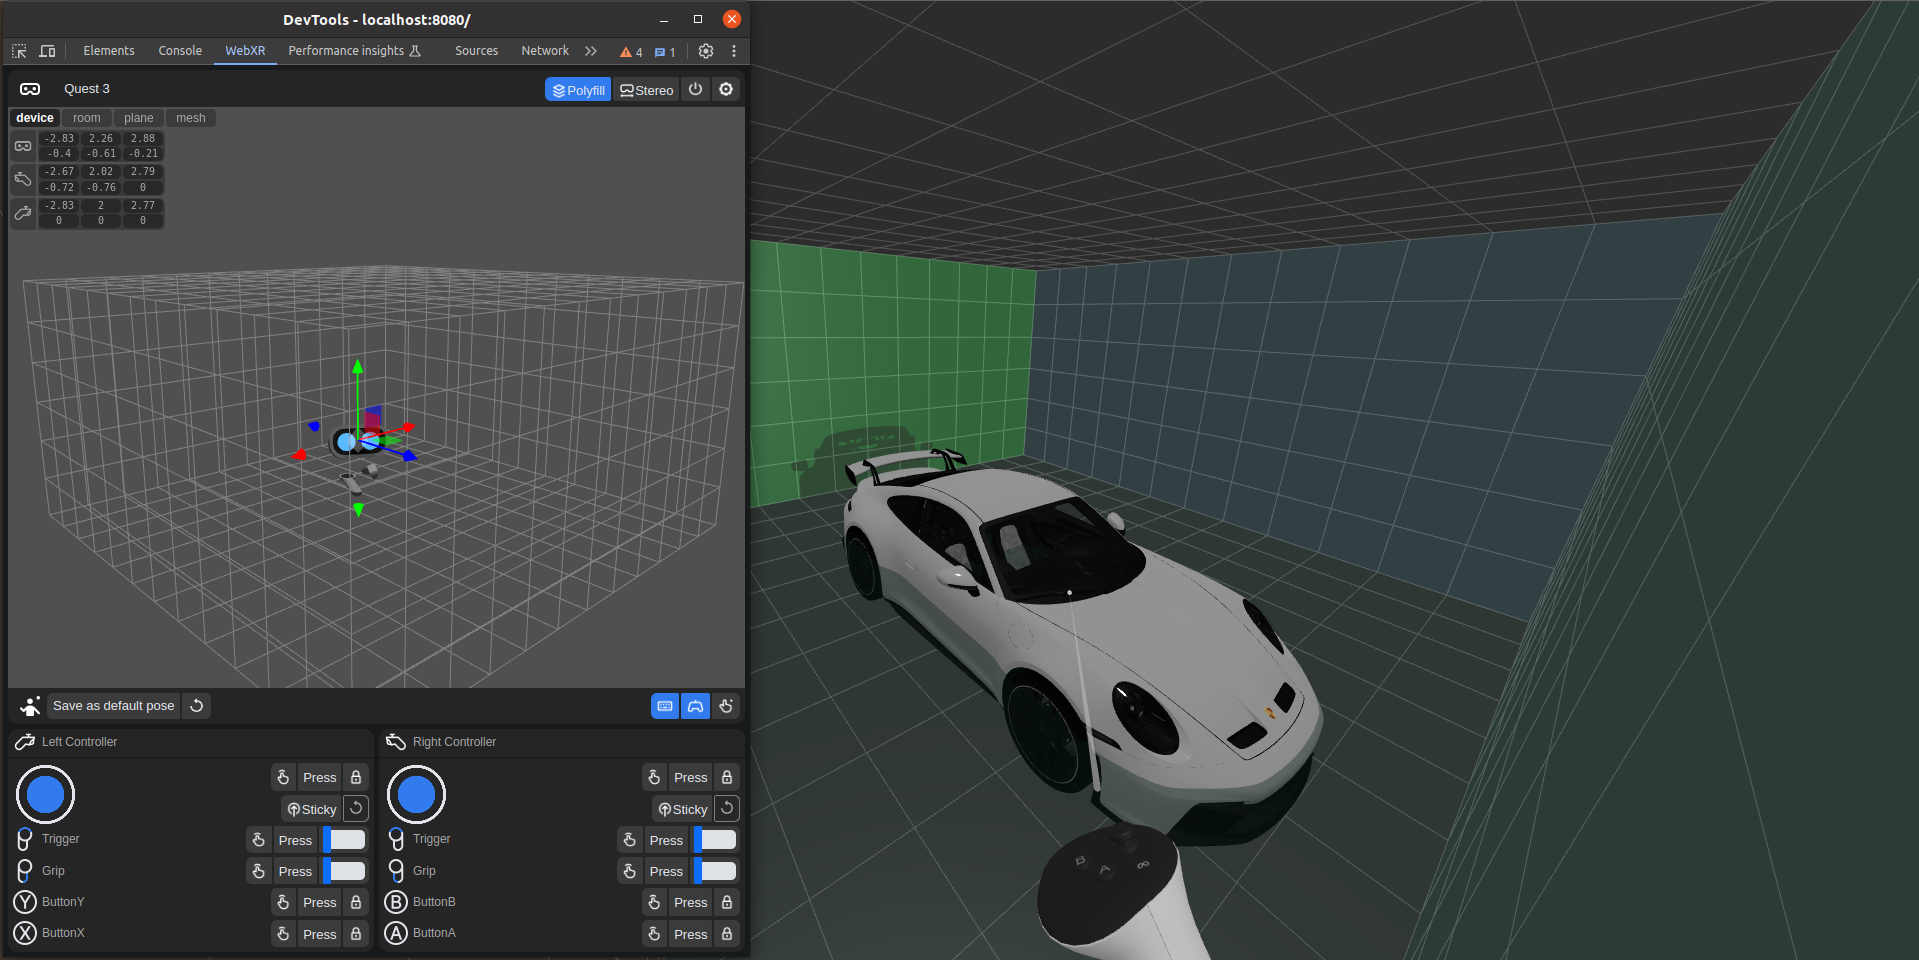
\includegraphics[width=0.7\textwidth]{images/WebXR-Emulator.png}
    \caption{Screenshots der Immersive Web Emulator Erweiterung in Chrome}
    \label{fig:webxr-emulator}
\end{figure}

Die Anwendung kann mit dieser Erweiterung deutlich schneller und einfacher getestet werden als mit der Meta Quest 3, da keine Verbindung zur Meta Quest 3 notwendig ist und die Anwendung direkt im Browser des Entwicklungsrechners getestet werden kann.
Des Weiteren sind die Ladezeiten beim Neuladen der Anwendung deutlich kürzer, da die Anwendung nicht auf die Übertragung der Daten auf die Meta Quest 3 warten muss.
Aufgrund der relativ großen Datenmengen, die für die Darstellung der 3D-Modelle erforderlich sind, ist der Unterschied der Ladezeiten zwischen Headset und Erweiterung signifikant.
Daher wurde jede neue Änderung zunächst im Emulator getestet, bevor die Anwendung im Headset neu geladen wurde.

Dennoch ist es von essenzieller Bedeutung, die Anwendung auch regelmäßig auf der Meta Quest 3 zu testen, da die Performance und die Interaktionen auf dem Emulator nicht immer exakt der Realität entsprechen.
So können beispielsweise leichte Ruckler auftreten, die durch eine unzureichende Optimierung der Anwendung bedingt sind.
Diese Ruckler sind nur bei der höheren Bildwiederholrate des Headsets sichtbar und können daher im Emulator nicht erkannt werden.
Daher wurde vor allem nach großen Änderungen des Prototyps stets auch mit dem AR-Headset selbst getestet.
Für kleinere Anpassungen, wie beispielsweise das Positionieren von Objekten, die häufig getestet werden müssen, wurde teilweise nur der Web-Emulator genutzt, um die lange Ladezeit zu vermeiden.
Die Vorgehensweise beim Testen ist im folgenden Diagramm in der Abbildung \ref{fig:webxr-entwicklung} zusammenfassend dargestellt.

\begin{figure}[H]
    \centering
    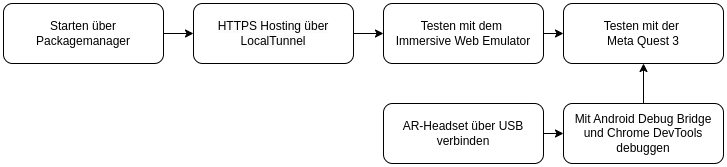
\includegraphics[width=1\textwidth]{images/WebXR-Entwicklung.png}
    \caption{Ablaufdiagramm des normalen Entwicklungsablaufs}
    \label{fig:webxr-entwicklung}
\end{figure}

\newpage

\section{Implementierung der Interaktionskonzepte}

Im Folgenden wird die Implementierung der zuvor beschriebenen Interaktionskonzepte erörtert.
In diesem Kontext werden grundlegende Konzepte sowie die für deren Implementierung relevanten Technologien vorgestellt und erläutert.
Des Weiteren werden Screenshots der implementierten Konzepte gezeigt und die Funktionsweise der Interaktionen beschrieben.
Schließlich werden auch die Herausforderungen und Probleme bei der Implementierung aufgezeigt und diskutiert.

Vor der Implementierung des Konzepts muss zunächst eine grundlegende WebXR"=Anwendung erstellt werden, die die Interaktionen mit dem Controller ermöglicht.
Als Basis hierfür dient das Skelett einer WebXR-Anwendung aus einer Artikelserie des Taikonauten-Magazins \autocite[][]{taikonauten-magazine}. 
Die Anwendung nutzt bereits die vom Nutzer gescannten Umgebungen, um einen virtuellen Raum zu erstellen, in dem die Interaktionen stattfinden.
Dabei werden Wände und Böden der Umgebung erkannt und als Mesh in die Szene eingefügt, um dem Nutzer eine Interaktion mit der realen Umgebung zu ermöglichen.
Zudem wurden bereits einige Interaktionen des Controllers, wie das Auswählen von Objekten durch Raycasting, implementiert, die als Basis für die Implementierung der Interaktionskonzepte dienen.

Da im Rahmen der Implementierung auch auf spezifische Knopfbelegungen des Controllers eingegangen wird, ist in Abbildung \ref{fig:controller-names} eine Darstellung eines rechten Meta Quest Touch Plus-Controllers mit den in dieser Arbeit genutzten Namen für die verschiedenen Bedienelemente.

\begin{figure}[H]
    \centering
    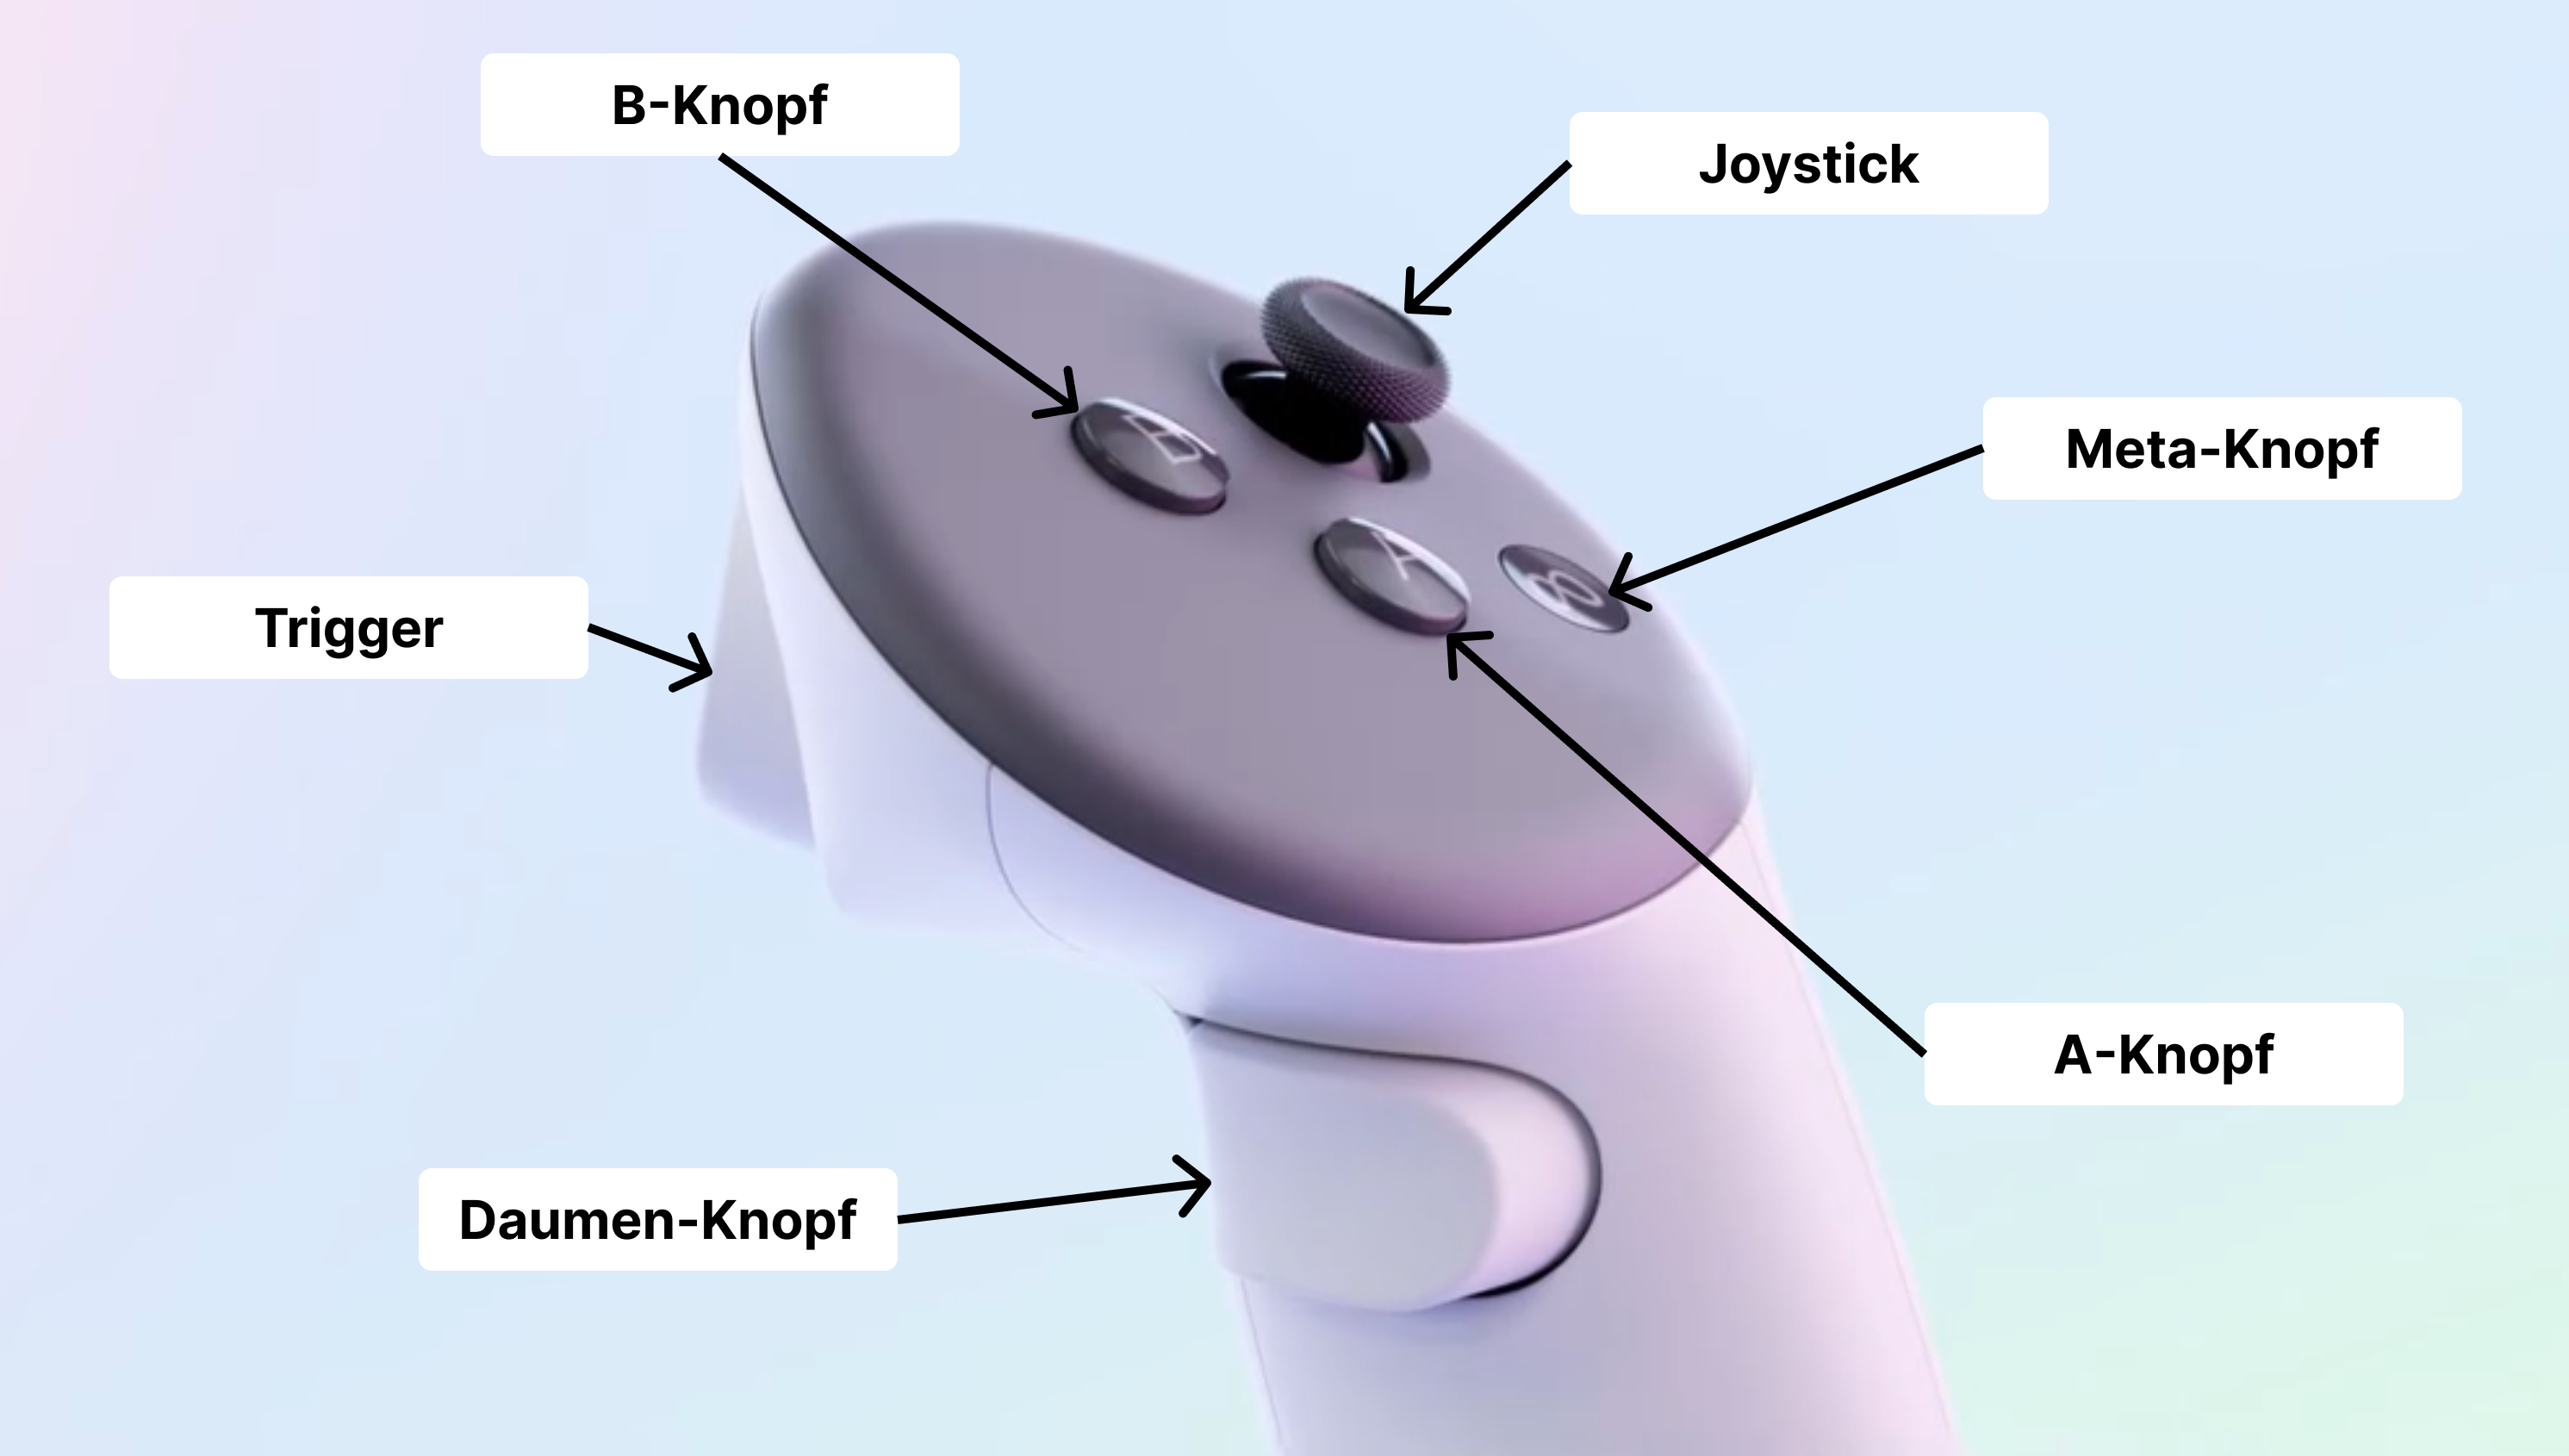
\includegraphics[width=0.8\textwidth]{images/QuestControllerButtons.png}
    \caption{Schema der Bedienelemente des Quest Controllers mit den im Rahmen dieser Arbeit genutzten Namen}
    \source{\autocite{meta-quest-3}}
    \label{fig:controller-names}
\end{figure}

\subsection{Explodierende Bauteile}

Der erste Schritt bei der Implementierung des Interaktionskonzepts der \glqq{}explodierenden\grqq{} Bauteile ist die Erstellung eines 3D-Modells, welches die Bauteile des Produkts enthält.
Jedes Bauteil muss dabei als eigenes Objekt im 3D-Modell vorhanden sein, damit es in der Animation separat dargestellt und referenziert werden kann.
Für die erste Implementierung wird ein einfaches 3D-Modell eines Tetris-Blocks verwendet, welcher aus vier verschiedenfarbigen Bauteilen besteht.
Basierend auf der Implementierung des Tetris-Blocks soll dann das Konzept auf ein komplexeres Modell, wie beispielsweise ein Fahrzeug, übertragen werden.

Das Modell wurde zunächst in Blender erstellt und als 3D-Modell im glTF-Format, welches wie WebXR von der Khronos Group entwickelt wurde, in die Anwendung exportiert.
Das glTF-Format ist ein offenes 3D-Dateiformat, welches für die effiziente Übertragung von 3D-Modellen im Web optimiert ist und die Dateigröße möglichst klein hält.
Ein weiterer Vorteil des glTF-Formats besteht darin, dass es auch Animationen und Materialien unterstützt, die im 3D-Modell enthalten sind.
So kann die Animation der Bauteile auch direkt in der Modellierungssoftware erstellt und in das glTF-Modell mit integriert bzw. eingebacken werden.
Dies ist von essenzieller Bedeutung für die effektive technische Umsetzbarkeit des Konzepts, da die Animation der Bauteile auf diese Weise in speziellen Animationsprogrammen, wie beispielsweise Blender, erstellt werden kann, ohne dass hierfür die WebXR-Anwendung selbst erforderlich wäre.
Dies ermöglicht die Erstellung komplexer Animationen, die nur mit den Tools von Babylon.js selbst nicht oder nur mit einem hohen Aufwand realisierbar wären.

Der nächste Schritt ist das Platzieren des erstellten 3D-Modells in der WebXR-Umgebung.
Das Prinzip des Raycastings wird verwendet, um dem Nutzer zu ermöglichen, mit dem Controller einen Punkt im Raum auszuwählen, an dem das 3D-Modell platziert werden soll.
Der Raum, in dem sich der Anwender befindet, muss dafür vor Beginn einmalig in den Meta Quest Einstellungen als Umgebung eingescannt werden.
Ist das geschehen, werden durch das Skelett der Anwendung des Taikonauten-Magazins bereits die Wände und Böden der Umgebung als Meshes erkannt und in die Szene eingefügt.
Anschließend wird durch den Controller ein Strahl in die Szene geschossen, wobei bei Knopfdruck des Triggers der Punkt, an dem der Strahl ein Objekt trifft, als Event zurückgegeben wird.

An dieser Stelle erfolgt die Definition eines Ankerpunktes, welcher vom 3D-Modell als Referenzpunkt im AR-Raum genutzt wird.
Der Ankerpunkt stellt ein Babylon.js-Objekt dar, welches in der Lage ist, einen Punkt im AR-Raum auch bei Bewegung des Nutzers am gleichen Ort zu halten.
Bewegt sich der Ankerpunkt, so bewegt sich auch das 3D-Modell mit, sodass es stets an der gleichen Stelle im Raum bleibt.

Nachdem das 3D-Modell platziert wurde, kann die Animation des Produkts gestartet werden.
Der A-Knopf des Controllers wird als Start-Button für die Animation genutzt, wobei die Wiedergabe vorwärts und rückwärts möglich ist.
Für die Animation wird die aus Blender in das glTF-Modell eingebackene Animation verwendet.
Dafür wird in Babylon.js eine Animationsfunktion erstellt, welche die Steuerung der Animation des Modells über einige Parameter, wie beispielsweise den Start- und Endframe der Animation, ermöglicht.
So kann für die Vorwärts- und Rückwärtsanimation die gleiche Funktion verwendet werden, indem die Start- und Endframe-Parameter basierend auf einem globalen Boolean, welcher den Animationsstatus speichert, gesetzt werden.

Beim Abspielen der Animation wird jedes Bauteil des Produkts in einer Schleife durchlaufen und dessen Animation gestartet.
Diese Schleife wird dann auch genutzt, um den einzelnen Bauteilen ihre Requirements als Text-UI-Elemente zuzuweisen.
Innerhalb der Schleife erfolgt zunächst eine Überprüfung, ob zu der jeweiligen ID des Bauteils Requirements existieren, die dargestellt werden sollen.
Sofern dies der Fall ist, wird in Babylon.js eine Fläche erstellt, auf welcher der Text dargestellt wird, und diese Fläche an das Bauteil als Kindobjekt angehängt.
Analog zum gesamten Modell, welches den Ankerpunkt als Referenzpunkt nutzt, nutzt jedes Requirement-Panel die Position seines Bauteils als Referenzpunkt für seine Position im AR-Raum.
Die Fläche kann zudem als Knopf fungieren, sodass bei Betätigung beispielsweise das Bauteil vergrößert oder eine Detailansicht des Bauteils aufgerufen werden kann.
Diese UI-Elemente werden jedoch, wie in Abbildung \ref{fig:tetris-explosion} zu sehen ist, nur angezeigt, wenn das Produkt gerade \glqq{}explodiert\grqq{} ist und nicht, wenn das Produkt sich gerade im Normalzustand befindet.

\begin{figure}[H]
    \centering
    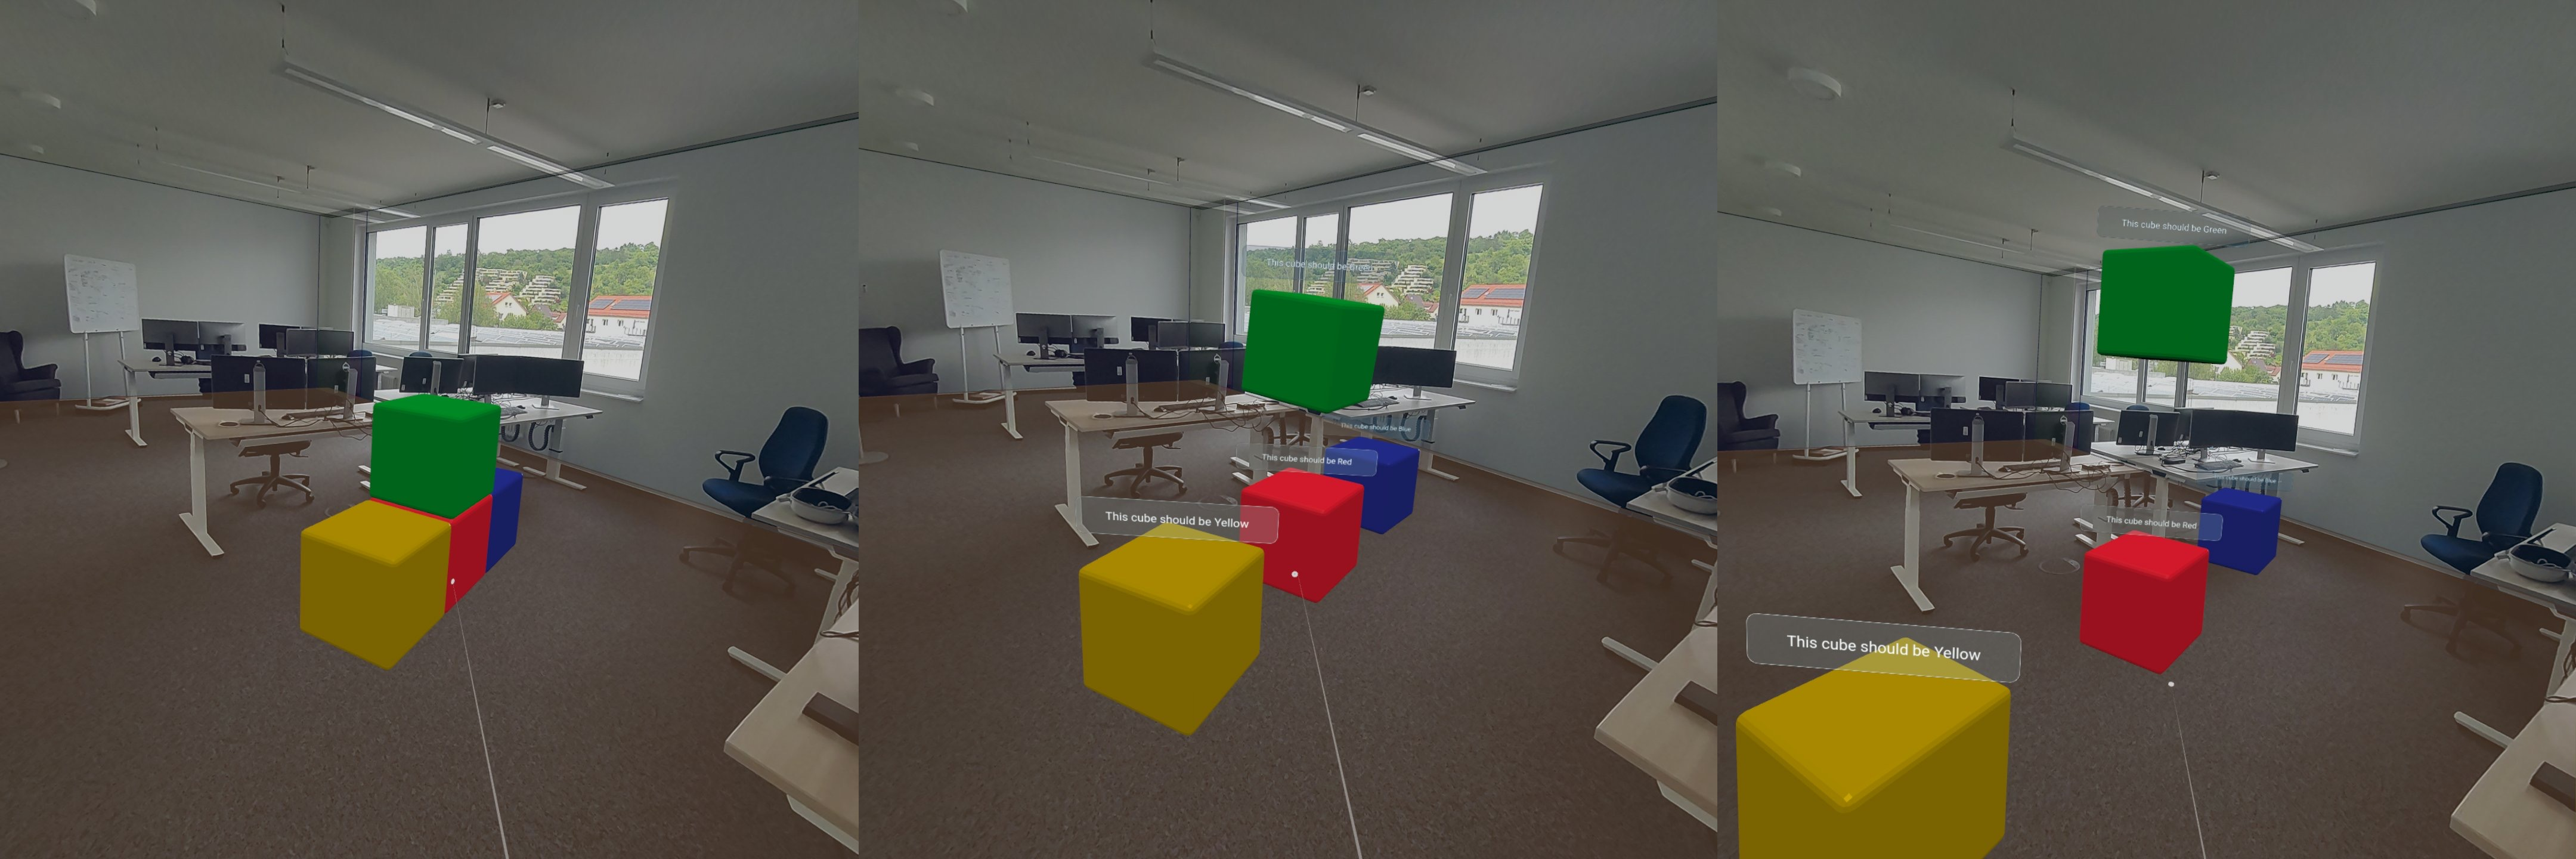
\includegraphics[width=1\textwidth]{images/tetris-explosion.png}
    \caption{Screenshots des explodierenden Tetris-Blocks mit Requirements in AR}
    \label{fig:tetris-explosion}
\end{figure}

\subsubsection{Implementierung an einem komplexeren Modell}

Nachdem das Interaktionskonzept funktionell am einfachen Modell eines Tetris-Blocks implementiert wurde, ist die nächste Herausforderung die Implementierung an einem komplexeren Modell.
Dafür wird ein relativ detailliertes 3D-Modell eines Porsche 911 von der 3D-Asset-Website Sketchfab verwendet, welches von dem Nutzer Abdul Azim Sharif erstellt und unter der CC BY 4.0 Lizenz veröffentlicht wurde \autocite[][]{SketchfabPorsche}.
\newpage
Das Modell, welches in Abbildung \ref{fig:porsche} dargestellt ist, wurde ausgewählt, da es eine Vielzahl an unterschiedlichen Bauteilen beinhaltet, die in der Animation separat dargestellt werden können.

\begin{figure}[H]
    \centering
    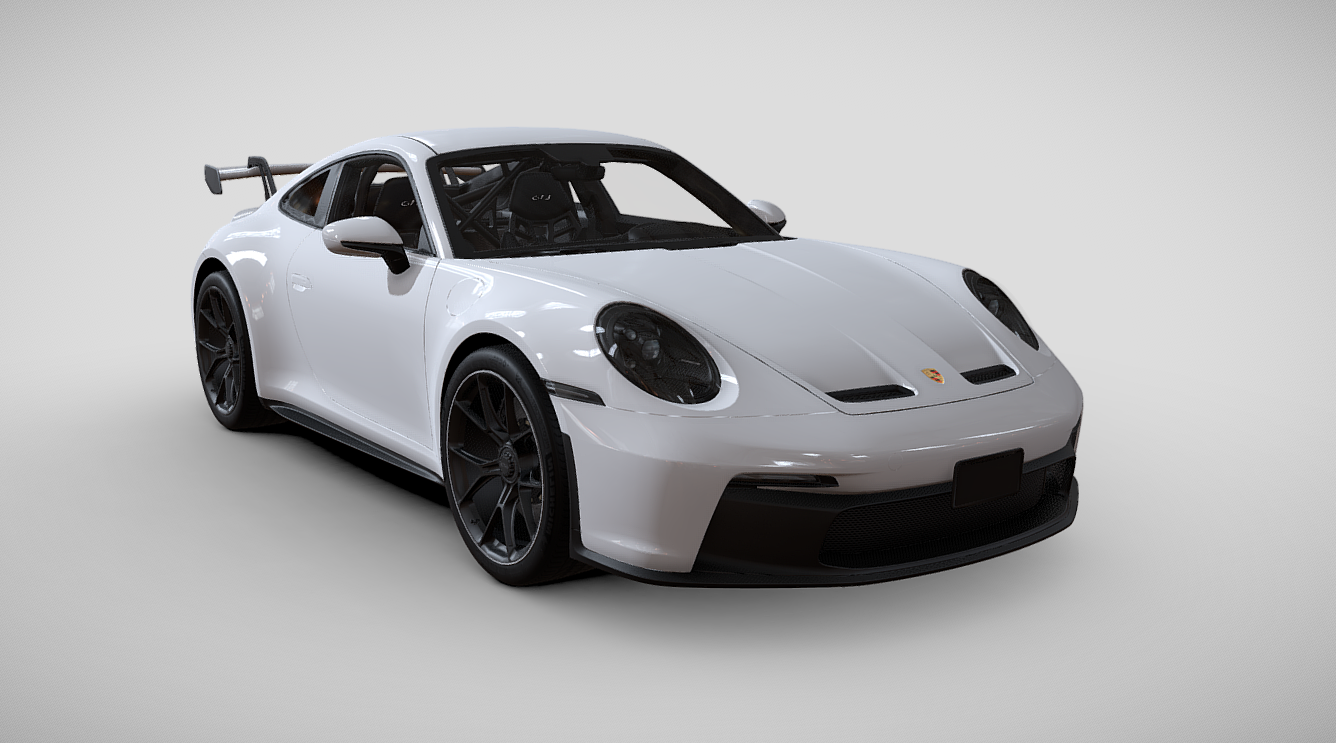
\includegraphics[width=0.8\textwidth]{images/PorscheModell.png}
    \caption{Screenshot des in der Anwendung genutzten Porsche Modells}
    \source{\autocite{SketchfabPorsche}}
    \label{fig:porsche}
\end{figure}

Bei dem in dieser Bachelorarbeit verwendeten Modell ist jedoch zu berücksichtigen, dass es sich nicht um ein vollständig akkurates und funktionales Modell eines Fahrzeugs handelt.
Beispielsweise existieren keine Achsen, an denen die Räder hängen.
Für die Zwecke dieser Bachelorarbeit ist das Modell jedoch ausreichend, da es eine hinreichende Anzahl an \glqq{}realen\grqq{} Bauteilen enthält, um das Interaktionskonzept anschaulich zu demonstrieren.
Würde das Interaktionskonzept in einer echten Anwendung für Kunden verwendet werden, sollte jedoch mit möglichst akkuraten CAD-Modellen gearbeitet werden, um die Requirements an die Bauteile möglichst genau darzustellen.

Für die Verwendung des Modells in der Anwendung muss als Nächstes eine Animation mit dem Modell erstellt werden, welche die Bauteile des Fahrzeugs in ihre Einzelteile zerlegt.
Dafür wird in Blender eine Animation erstellt, welche einige Bauteile, wie beispielsweise die Verkleidung, die Räder und den Spoiler, nach außen wegbewegt.
Beim Erstellen der Animation musste zudem beachtet werden, dass sich möglichst wenig Bauteile bei der Animation überschneiden.
Infolgedessen haben einige Bauteile eine sehr einfache Animation mit lediglich zwei Keyframes, beispielsweise die Räder, welche lediglich nach außen verschoben werden.
Andere Bauteile hingegen erfordern eine komplexere Animation mit bis zu fünf Keyframes, um Überschneidungen zu vermeiden.

\newpage

Zur Veranschaulichung der Animation ist in Abbildung \ref{fig:porsche-explosion} eine Bildsequenz der Animation des Porsche-Modells zu sehen.

\begin{figure}[H]
    \centering
    \includegraphics[width=1\textwidth]{images/PorscheExplosion.png}
    \caption{Bildsequenz der Animation des Porsche Modells}
    \label{fig:porsche-explosion}
\end{figure}

Um den Bauteilen später ihre Requirements zuzuweisen, ist es erforderlich die relevanten Bauteile identifizierbar zu machen.
Zu diesem Zweck wird in Blender jedem animierten Objekt zu Beginn des Objektnamens eine ID zugewiesen, beispielsweise \glqq{}\#1\_Rad\grqq{} oder \glqq{}\#2\_Lichter\grqq{}.
Diese ID dient im späteren Verlauf als Referenz für die Requirements.

Die IDs werden dabei zusätzlich in anzeigende und nicht-anzeigende IDs unterteilt, um bei Bauteilen welche aus mehreren kleinen Objekten bestehen in der großen Ansicht nur die Requirements des Hauptobjekts anzuzeigen.
Beispielsweise besteht ein Rad aus Reifen, Felge, Bremsscheibe etc., wobei dann nur der Reifen als Requirements an das gesamte Rad anzeigt und die anderen Objekte die Requirements an sich selbst in der Detailansicht.
Um eine einfache Zuordnung der Objekte zu ihren Elternobjekten zu ermöglichen, beispielsweise für die Klick-Abfrage des Rads, werden die IDs der Elternobjekte in den IDs der Kindobjekte gespeichert.
Dabei wird jedoch auf die Verwendung eines Unterstrichs \glqq{}\_\grqq{} hinter der ID verzichtet, wodurch sie beim Erstellen der Requirementpanels herausgefiltert und ignoriert werden können.

Die detaillierte Radansicht stellt ein separates, ebenfalls in Blender erstelltes glTF-Modell dar, welches lediglich das Rad, seine Bauteile sowie die darin eingebetteten Animationen umfasst.
Im Rahmen der Implementierung der detaillierten Radansicht wird eine Abfrage hinzugefügt, welche prüft, ob der Nutzer mit seinem Controller auf ein Rad klickt.
Die Bestimmung des Punktes, an dem der Controller auf ein Objekt trifft, erfolgt wiederum gemäß dem Raycasting-Prinzip.
Sofern das getroffene Objekt Teil des Rads ist, also die ID des Rads enthält, wird an der betreffenden Stelle ein neuer Ankerpunkt definiert, an dem die Detailansicht des Rads angezeigt wird.
In der Folge werden der bisherige Ankerpunkt sowie die Bauteile des Fahrzeugs ausgeblendet, während die Bauteile des Rads an den neuen Ankerpunkt angehängt werden.
Bei einem erneuten Wechsel zur Gesamtansicht des Fahrzeugs wird das Fahrzeugmodell wieder an den Ankerpunkt angehängt, während die Detailansicht des Rads ausgeblendet wird.
Auf diese Weise kann der Nutzer die Requirements an das Rad in einer Detailansicht betrachten und bei Bedarf wieder zur Gesamtansicht des Fahrzeugs zurückkehren.

\subsection{Wolken von Requirements}

Das Interaktionskonzept der Wolken aus Requirementpanels ist im Vergleich zum Konzept der explodierenden Bauteile deutlich einfacher zu implementieren, da kein zugehöriges Modell oder eine individuelle Animation benötigt wird.

Im Rahmen der Implementierung wurde zunächst ein einfacher Algorithmus entwickelt, der einen Array von Requirements erhält und zu diesen eine 3D-Wolke von Punkten in einem gegebenen Bereich erstellt.
Der ursprüngliche Algorithmus generiert, wie im Ablaufdiagramm in Abbildung \ref{fig:wolken-algo} dargestellt, einen etwas zu großen Array aus 3D-Punkten in Form eines Würfels.
In der Folge wird aus der Mitte des Punktearrays ein Teilarray in der Länge des Requirementarrays genutzt, um UI-Panels mit den Requirements an den jeweiligen Punkten zu platzieren.
Dafür werden die Requirements eines Clusters in einer Schleife durchlaufen, wobei für jedes Requirement ein UI-Panel mit dem Text des Requirements an der Stelle des zugehörigen Punktes des Punktearrays erstellt wird.

Die Skalierung der Abstände der Punkte wurde durch das Testen verschiedener Abstände mit einfachen Beispielpanels bestimmt und kann auch über den Algorithmus selbst angegeben werden.
Auf diese Weise sollte das Clipping, also das Kollidieren von nebeneinanderliegenden Panels, verhindert werden.

\begin{figure}[H]
    \centering
    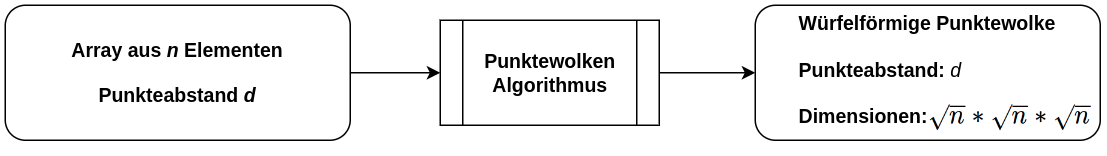
\includegraphics[width=1\textwidth]{images/WolkenAlgo.png}
    \caption{Funktionsweise des Punktewolken Algorithmus}
    \label{fig:wolken-algo}
\end{figure}


Wie beim Konzept der explodierenden Bauteile wird auch hier ein Ursprungspunkt der Wolken durch Raycasting und Auslösen des Triggers des Controllers bestimmt.
Die Wolken sollen dann über dem Punkt, der auf dem Boden ausgewählt wurde, schweben.
Dafür werden die Textpanels beim Erstellen etwas nach oben verschoben.

\newpage

Eine erste Betrachtung der Requirements in Wolken zeigte jedoch, dass sich die Textpanels bereits in kleinen Wolken stark überlappen und viele Requirements so nur schwer bis gar nicht lesbar sind.
Wie in Abbildung \ref{fig:wolken-prototyp} zu sehen ist, treten bereits bei Wolken von fünf Requirements starke Überlappungen auf, welche die Lesbarkeit der Requirements stark beeinträchtigen.

\begin{figure}[H]
    \centering
    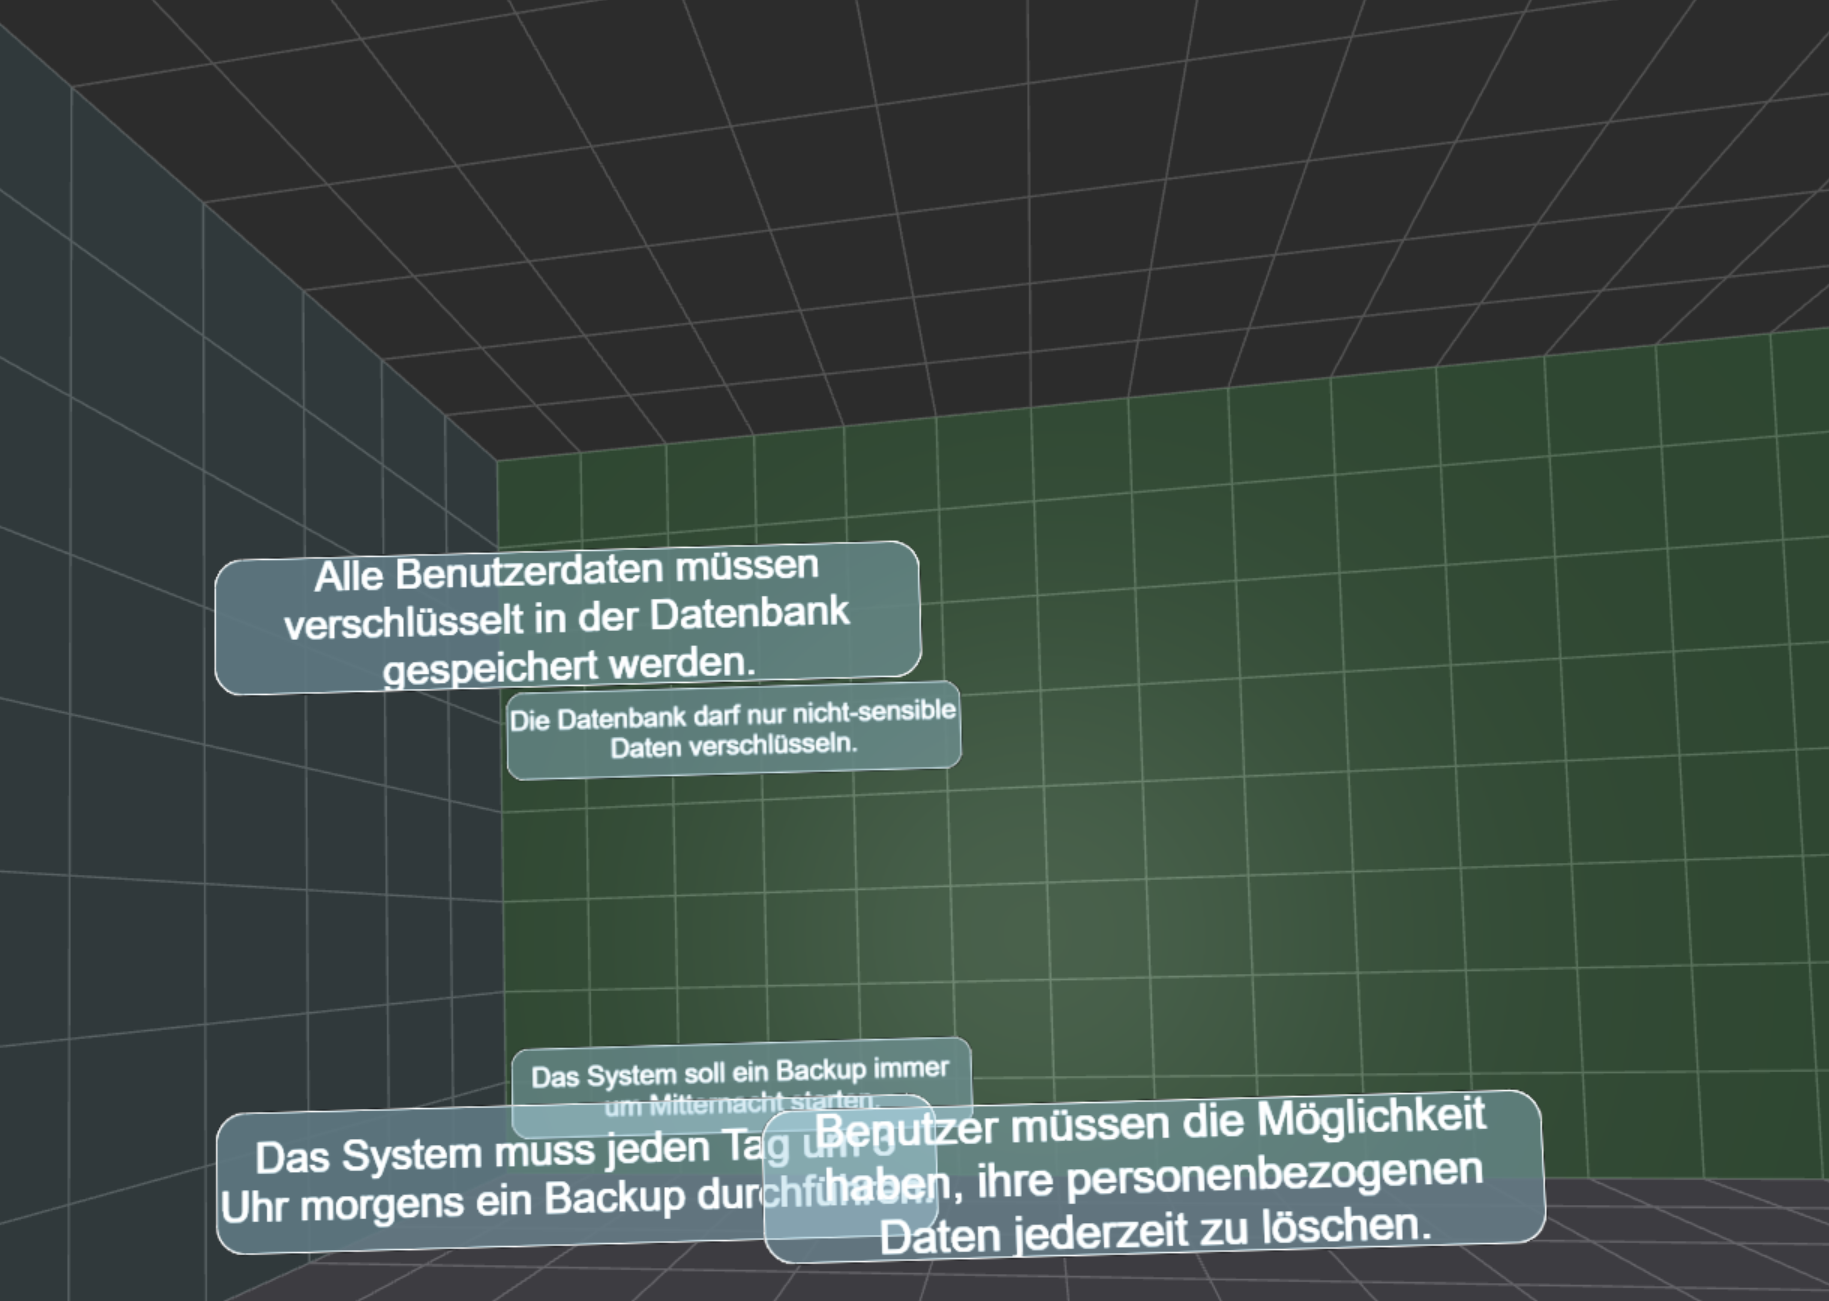
\includegraphics[width=0.8\textwidth]{images/WolkenPrototyp.png}
    \caption{Wolke aus 5 Requirementpanels}
    \label{fig:wolken-prototyp}
\end{figure}

In Abbildung \ref{fig:wolken-prototyp} wird ersichtlich, dass die Transparenz der UI-Elemente dazu führt, dass Überlappungen auch die vordersten Requirements unlesbar machen.
Daher war die erste Änderung, die UI-Elemente undurchsichtig zu machen, um zumindest die Lesbarkeit der vordersten Elemente zu gewährleisten.
Des Weiteren wurde der Abstand der Requirement-Panels zueinander vergrößert und die Requirements wurden mittels einer Zufallsfunktion jeweils leicht von ihrem Ursprungspunkt verschoben, um die Überlappungen zu reduzieren.
Der Algorithmus, der die Punktewolke generiert, wurde zusätzlich noch so wie in Abbildung \ref{fig:wolken-algo-ang} dargestellt angepasst, damit er keine würfelförmigen Punktewolken mehr erstellt, sondern diese Würfelform etwas abflacht, um Wolken in Form eines Quaders zu erhalten.
Bei kleinen Requirementwolken resultieren die vorgenommenen Anpassungen in einer verbesserten Lesbarkeit der Requirements, wobei die meiste Zeit nahezu alle Requirements lesbar sind.

\begin{figure}[H]
    \centering
    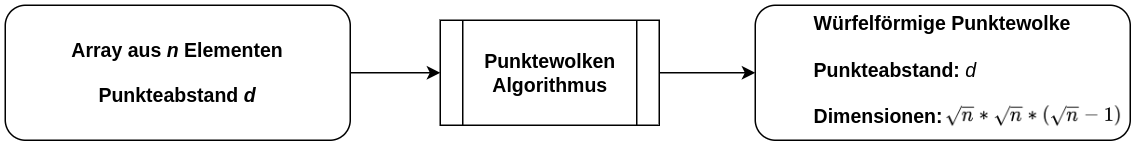
\includegraphics[width=1\textwidth]{images/WolkenAlgoAngepasst.png}
    \caption{Funktionsweise des angepassten Punktewolken Algorithmus für flachere Wolken}
    \label{fig:wolken-algo-ang}
\end{figure}

\newpage

Allerdings lässt sich bereits bei einer geringfügig größeren Requirementwolke, wie sie in Abbildung \ref{fig:wolken-prototyp-3} dargestellt ist, erkennen, dass sich Überlappungen bei realistischen Wolkengrößen nicht gänzlich vermeiden lassen. 

\begin{figure}[H]
    \centering
    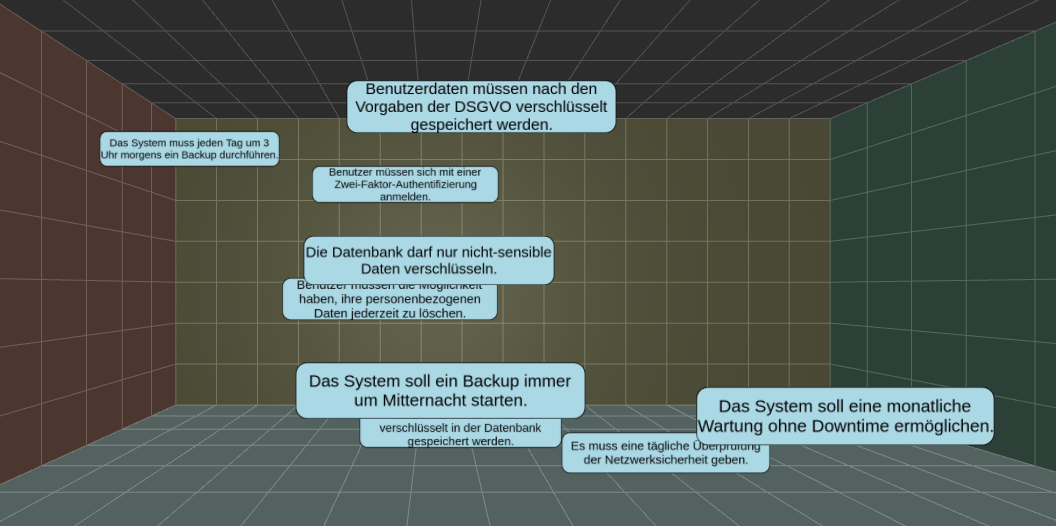
\includegraphics[width=0.9\textwidth]{images/WolkenPrototyp3.png}
    \caption{Wolke aus 9 Requirements mit undurchsichtigen Panels und größerem Abstand}
    \label{fig:wolken-prototyp-3}
\end{figure}

Insofern lässt sich festhalten, dass das Konzept trotz initialer Anpassungen noch immer mit einer signifikanten Beeinträchtigung der Lesbarkeit und damit der Usability der Darstellung zu kämpfen hat.
Das Interaktionskonzept der Wolken war insbesondere für die Bearbeitung umfangreicher Mengen an Requirements konzipiert, weshalb die Usability der Darstellung auch bei großen Mengen von Requirements gewährleistet sein muss.
Um die Lesbarkeit der Requirements auch in großen Wolken zu optimieren, wurden drei alternative Ansätze evaluiert, die im Folgenden erörtert werden.

Der erste Ansatz zielte darauf ab, die Requirements mithilfe des Raycasting des Controllers zu fokussieren.
Auf diese Weise könnten Requirements, die gelesen werden sollen, in den Fokus gebracht und somit lesbar gemacht werden.
Jedoch wird bei diesem Ansatz der Überblick über alle Requirements nicht gewährleistet, da nur ein Requirement gleichzeitig fokussiert werden kann.
Zudem kann es bei großen Requirementwolken sein, dass gesuchte Requirements gar nicht gefunden und daher auch nicht fokussiert werden können, da sie durch andere Requirements verdeckt sind.
Bei Berücksichtigung der Tatsache, dass dieses Interaktionskonzept insbesondere für die gleichzeitige Darstellung einer Vielzahl von Requirements konzipiert wurde, erweist sich dieser Lösungsansatz als nicht geeignet.

Der zweite Ansatz zielte auf eine Verkleinerung der Requirementpanels ab, um eine größere Anzahl von Requirements in einer Wolke darstellen zu können.
Allerdings wurde bei dieser Vorgehensweise die Lesbarkeit der Requirements zum Problem.
Aufgrund des in Kapitel \ref{section:hmds} beschriebenen Screen-Door-Effekts und anderer Probleme bei der Schärfe von AR-Displays ist es schwierig, kleine Texte in AR gut lesbar darzustellen.
Dieses Problem der Unlesbarkeit wird bei großen Requirementwolken, in denen viele Requirements dargestellt werden, noch verstärkt, da diese auch einen größeren Raum abdecken müssen und so einige Requirements weit vom Nutzer entfernt sind.
Diese Probleme der Unschärfe durch Nähe zum Bildschirm treten jedoch bei modernen, konventionellen zweidimensionalen Bildschirmen aufgrund des Betrachtungsabstands nicht auf.
Dadurch ist eine Darstellung mit einer deutlich höheren Informationsdichte möglich.
Folglich erweist sich auch dieser Lösungsansatz als ungeeignet, um eine Vielzahl von Requirements gleichzeitig in einer geeigneten Form darzustellen.

Der dritte Ansatz bestand in der weiteren Entzerrung der Requirements, wobei die Requirements möglichst breitflächig ausgerichtet wurden, um Überlappungen zu vermeiden.
In der Folge wurde der Algorithmus dahingehend modifiziert, dass flachere, dafür aber breitere und höhere Punktewolken generiert werden.
Umso mehr Requirements dabei existieren, desto flacher sollte die Wolke werden um alle Requirementpanels gleichzeitig sichtbar zu machen.
Dieser Ansatz führt jedoch, wie in Abbildung \ref{fig:wolken-algo-ang2} dargestellt, in seiner letztem Konsequenz bei großen Wolken zu einer Darstellung aller Requirements auf einer zweidimensionalen Ebene.
Allerdings ist das Navigieren über große Flächen in AR unpraktisch im Vergleich mit einer ähnlichen Darstellung auf einem normalen Bildschirm.
Daher wird durch diesen Lösungsansatz die Darstellung der Requirements im dreidimensionalen Raum und in AR weniger effizient als in einer 2D-Darstellung.
Wenn die Wolken auch in AR in eine zweidimensionale Form gebracht werden, kann auch direkt eine zweidimensionale Darstellungsform gewählt werden.

\begin{figure}[H]
    \centering
    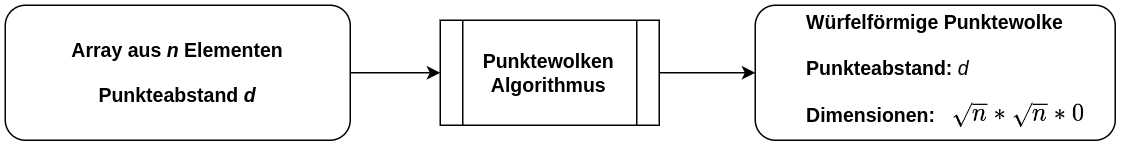
\includegraphics[width=1\textwidth]{images/WolkenAlgoAngepasst2.png}
    \caption{Extremversion eines abgeflachten Algorithmus zur Erstellung einer Punktewolke}
    \label{fig:wolken-algo-ang2}
\end{figure}

Die Analyse der vorliegenden Ansätze zeigt, dass keiner der Ansätze eine Lösung für das Problem der Überlappung und Lesbarkeit der Requirements bietet, welches das Konzept nicht weniger sinnvoll macht als eine 2D-Darstellung.
Daher wird das Konzept der Wolken von Requirements in AR nicht weiter verfolgt.

Im folgenden Kapitel \ref{section:2d} wird zur Untersuchung des Konzepts in 2D ein Mockup erstellt und analysiert.
Die darauf basierende Möglichkeit der Implementierung des Konzepts als 2D-Anwendung wird zudem noch im Ausblick in Kapitel \ref{section:ausblick} erörtert.

\newpage

\subsection{2D-Mockup für Wolken aus Requirements}
\label{section:2d}

Zur Veranschaulichung der Darstellung des Interaktionskonzepts der Requirementwolken wurden im UI-Prototyping-Tool Figma Mockups erstellt, welche die Wolken in einer Desktop-Anwendung visualisieren.
Im Folgenden werden anhand einiger Screenshots der Mockups die Unterschiede zur Darstellung in AR erörtert.
Der Fokus liegt dabei auf dem Vergleich der Usability der beiden Darstellungsformen.


Im ersten Screenshot aus Abbildung \ref{fig:wolken-2d-1} ist eine Übersicht über eine große Anzahl an Requirements dargestellt.
Da auch auf einem herkömmlichen Display lediglich eine begrenzte Anzahl von Requirements gleichzeitig dargestellt werden kann, werden die Requirements in der Übersicht abstrakt vereinfacht als Punkte ohne Textinhalt präsentiert. 
Jeder Punkt stellt dabei ein Requirement dar, die durch den Nutzer gelesen werden kann, sobald dieser auf das entsprechende Element hereinzoomt.

\begin{figure}[H]
    \centering
    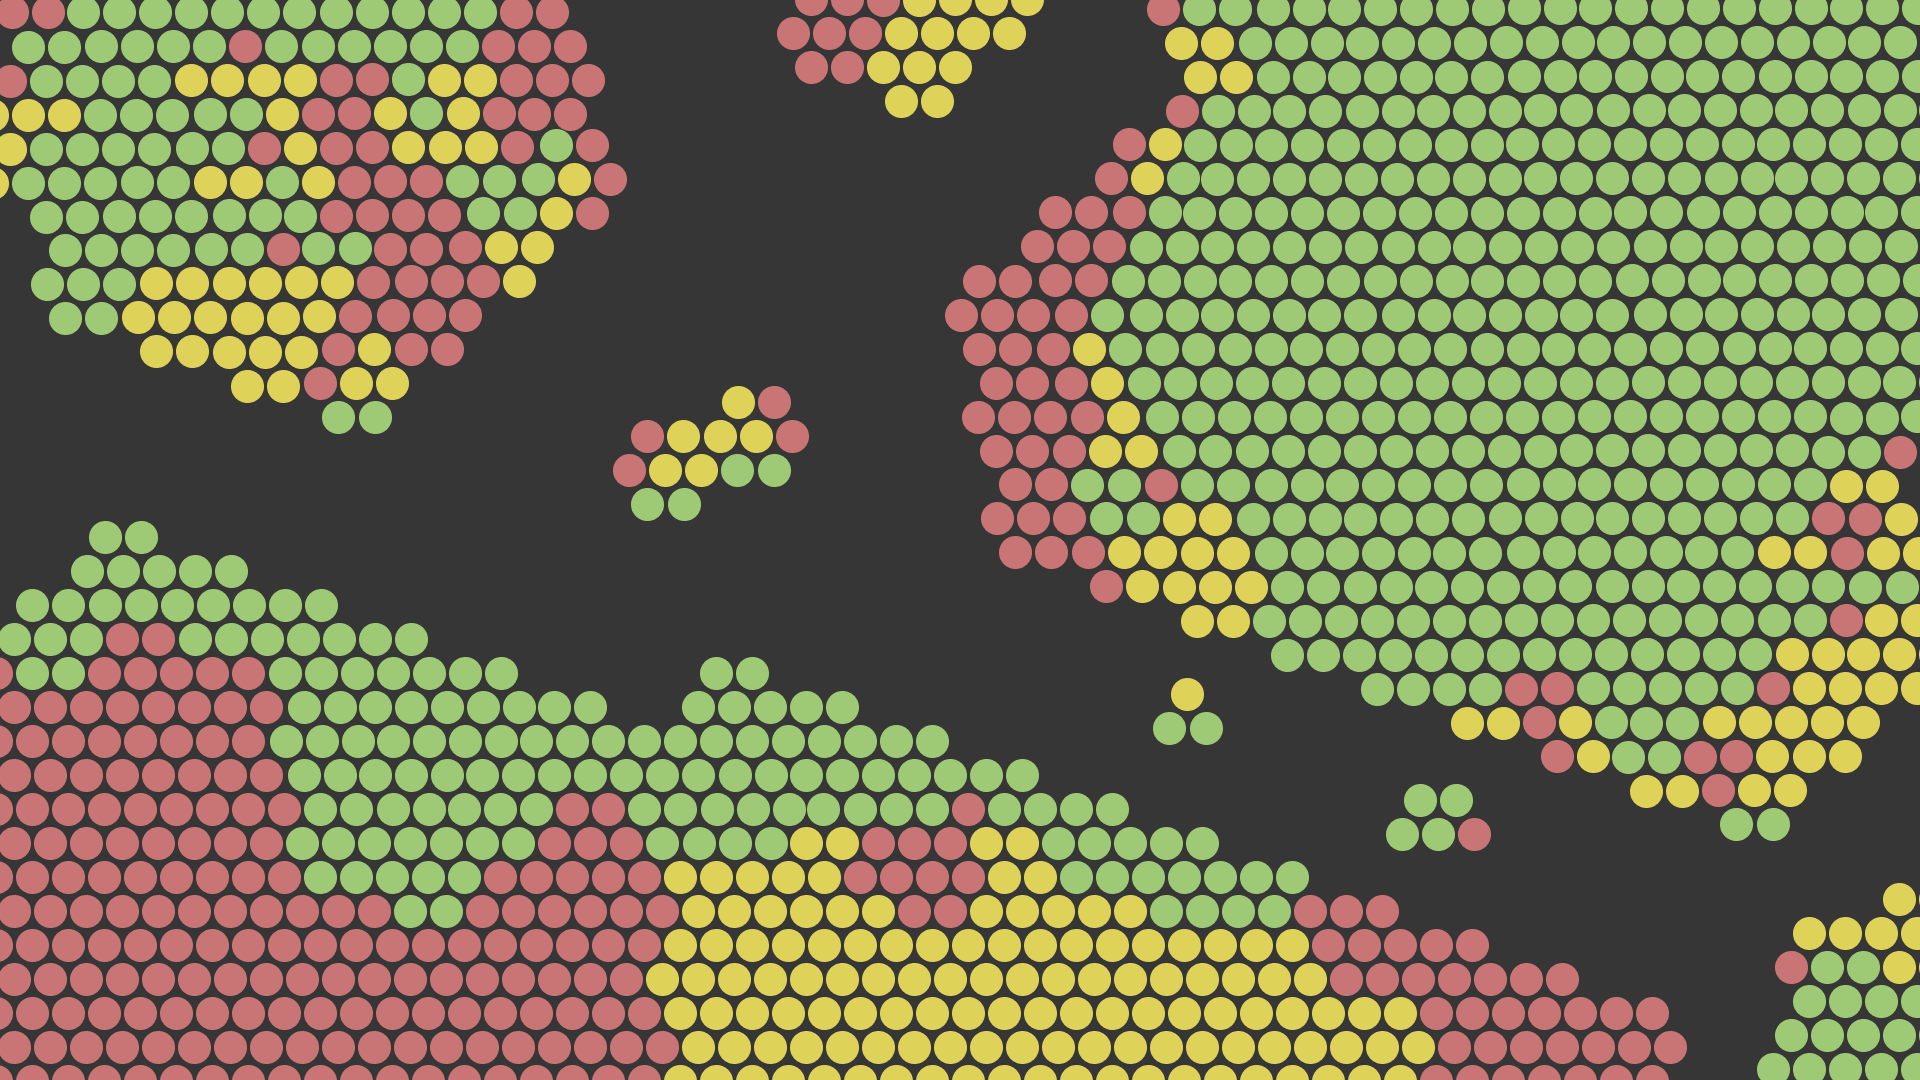
\includegraphics[width=1\textwidth]{images/FigmaWolkenOverview.png}
    \caption{Mockup zur Übersicht über eine große Anzahl an Requirements}
    \label{fig:wolken-2d-1}
\end{figure}

\newpage

Die Farben der Requirements dienen der visuellen Darstellung des jeweiligen Bearbeitungsstatus.
Dadurch wird eine unmittelbare Einordnung der Requirements ermöglicht.
\begin{itemize}
    \item \textbf{Grüne Requirements:} Die Requirements dieser Farbe wurden bereits vollständig bearbeitet und überprüft, sodass eine weitere Bearbeitung aktuell nicht erforderlich ist.
    \item \textbf{Rote Requirements:} Rote Requirements wurden noch nicht bearbeitet, sie sind meist neu oder wurden lang ignoriert.
    \item \textbf{Gelbe Requirements:} Requirements in gelber Farbe wurden bereits einmal bearbeitet, bedürfen jedoch noch einer Überprüfung. Alternativ könnten in dieser Farbe alte Requirements mit neuen Änderungen dargestellt werden.
\end{itemize}
Es wäre auch denkbar, die Farben auf andere Filter anzupassen.
Beispielsweise könnten Requirements mit der gleichen Farbe ein gleiches Bauteil betreffen.
Die Implementierung farbbasierter Filter in der Anwendung könnte zu einer weiteren Steigerung der Übersichtlichkeit der Requirements beitragen.

Die dargestellte Farbenkorrelation erlaubt eine einfache Erkennung von Bereichen, in denen noch Verwaltungsarbeit zu erledigen ist.
Zwar können offensichtlich nicht alle Requirements gleichzeitig mit ihrem Text betrachtet werden, doch durch die Vereinfachung der einzelnen Requirements als kleine Kreise ohne Text lässt sich ein gutes Gesamtbild erlangen.


Will man dann einzelne Requirements betrachten und mit diesen interagieren, kann in die Ansicht nahtlos hereingezoomt werden, um ab einer gewissen Größe die Requirement-Texte lesen zu können.
Wollen Nutzer auch nach spezifischen Requirements direkt suchen, ließe sich auch eine Suchfunktion einbauen, mit welcher direkt nach einzelnen Requirements bspw. anhand ihres Textes gesucht werden kann.
Die Größe, ab der die Texte als lesbar empfunden werden, ist dabei von den genutzten Bildschirmen sowie einigen weiteren nutzerspezifischen Eigenschaften abhängig.
Sie kann jedoch flexibel und intuitiv durch das Zoomen durch den Nutzer angepasst werden.

\newpage

In Abbildung \ref{fig:wolken-2d-2} ist ein Mockup einer hereingezoomten Perspektive dargestellt.
Hier können dann alle Texte der Requirements selbst gelesen werden und es können einzelne Requirements angeklickt werden, um weiter mit ihnen zu interagieren.
Denkbar wären auch Seitenmenüs, die sich beim Anklicken eines Requirements öffnen und detaillierte Informationen sowie eventuelle Interaktionsmöglichkeiten zu den Requirements anzeigen. 

\begin{figure}[H]
    \centering
    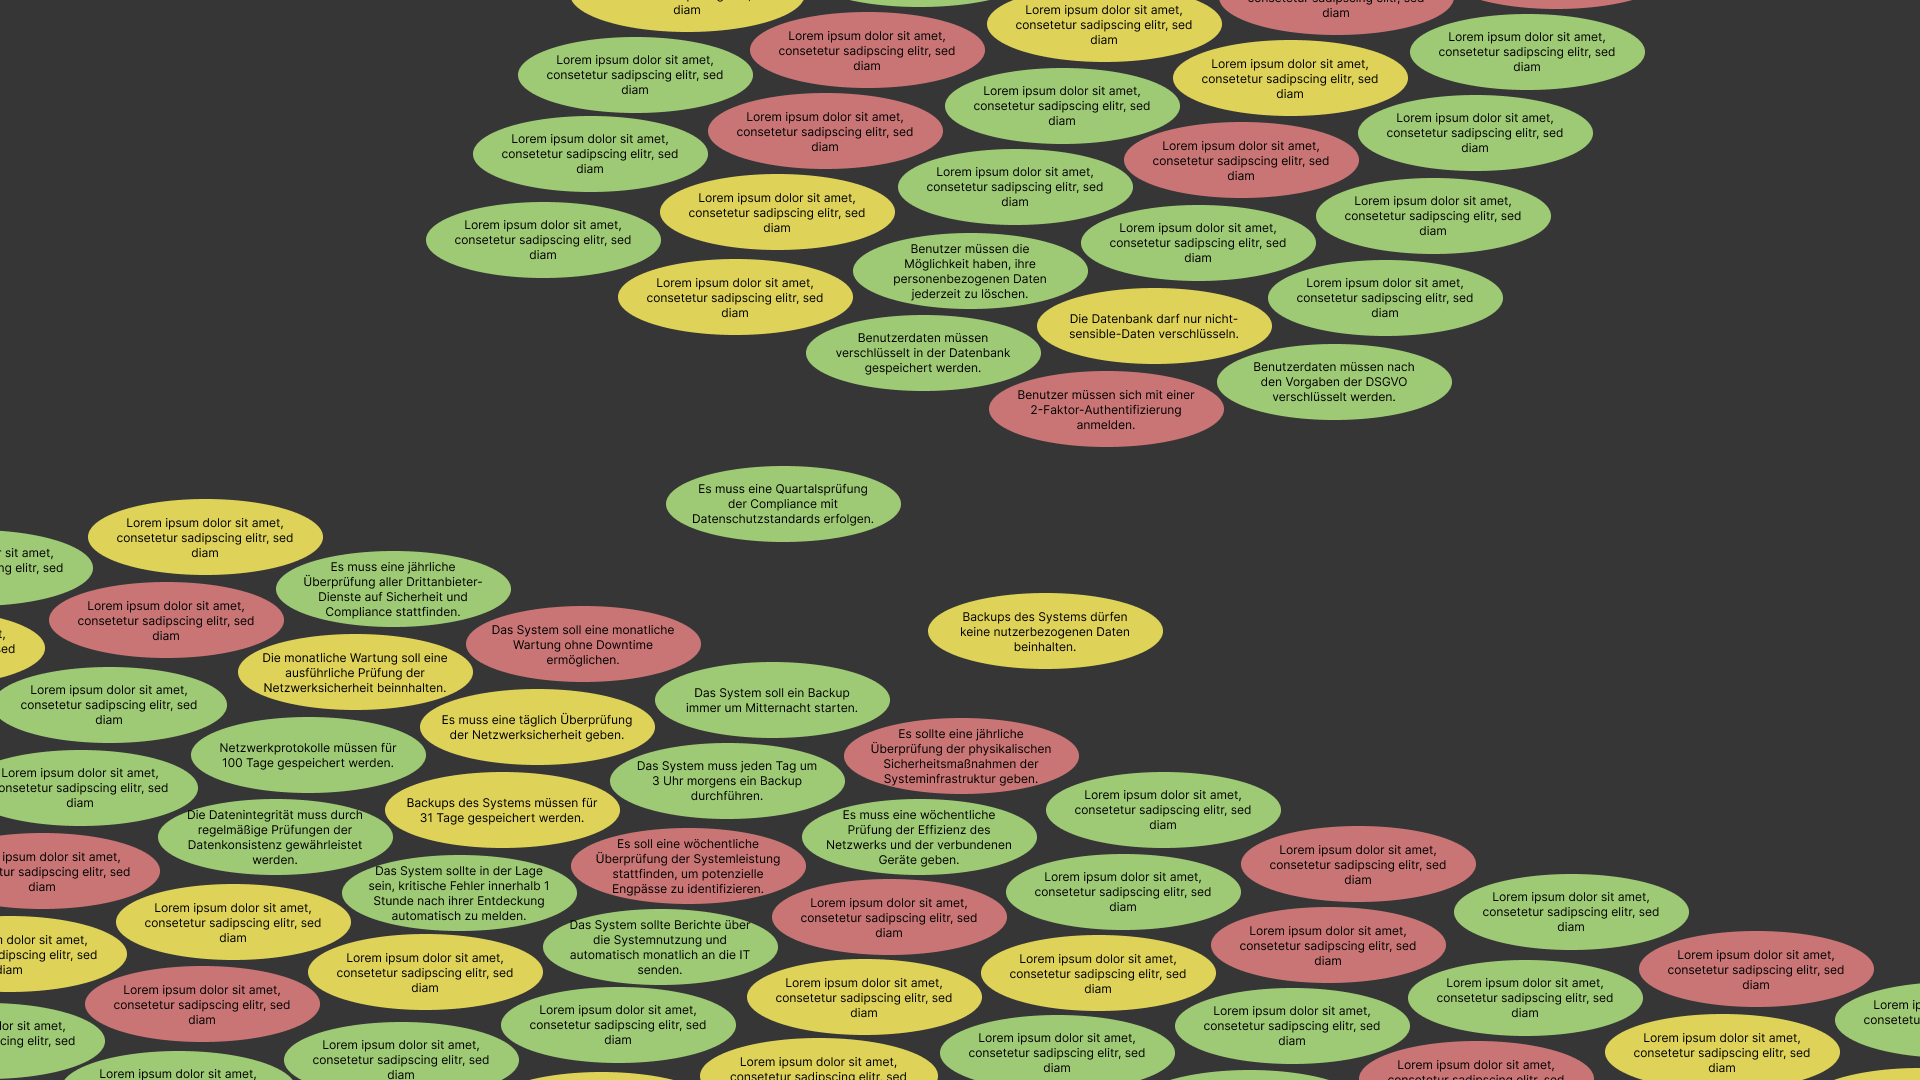
\includegraphics[width=1\textwidth]{images/FigmaWolkenCloseup.png}
    \caption{Mockup der hereingezoomten Ansicht}
    \label{fig:wolken-2d-2}
\end{figure}

Bei der Erstellung eines Mockups des Wolken-Interaktionskonzepts in 2D wurde ersichtlich, dass das Konzept zumindest bei erster Betrachtung keine nennenswerten Nachteile durch den Wechsel auf eine zweidimensionale Darstellung erfährt.

Tatsächlich lassen sich, wie in Abbildung \ref{fig:wolken-2d-1} gezeigt, durch die höhere mögliche Informationsdichte in der zweidimensionalen Darstellung sogar größere Wolken aus Requirements darstellen als in AR.
Obwohl durch die Abstraktion der Requirements als Punkte auch in AR eine deutlich größere Anzahl von Requirements dargestellt werden könnte, wäre dies nicht so effizient wie in 2D.
Schon durch die höhere Schärfe der meisten Displays durch den größeren Abstand des Nutzers im Vergleich zu HMDs können in einer klassischen, zweidimensionalen Anwendung deutlich kleinere Datenpunkte unterschieden werden.

In AR ist zu berücksichtigen, dass sehr kleine Elemente mit einem Controller schwieriger auszuwählen sind, als mit einer Maus.
Dies liegt daran, dass eine Maus auf einer statischen Fläche abgelegt wird, während der Controller frei in der Luft gehalten werden muss.
Aufgrund der genannten Eigenschaften ist zu erwarten, dass das Interaktionskonzept in 2D eine Verbesserung der Usability ermöglicht, insbesondere im Hinblick auf das Zielen mit einer Maus auf kleine Elemente.

% DeepL korrigiert